\documentclass[11pt,a4paper]{article}
\usepackage[margin=25mm]{geometry}
\usepackage[T1]{fontenc}
\usepackage{lmodern,microtype,amsmath,amssymb,graphicx,booktabs,tabularx,array,makecell,float,placeins,xurl}
\usepackage[colorlinks=true,linkcolor=blue,urlcolor=blue]{hyperref}
\renewcommand{\thesection}{S\arabic{section}}
\renewcommand{\thetable}{S\arabic{table}}
\renewcommand{\thefigure}{S\arabic{figure}}
\setlength{\emergencystretch}{2em}
\title{Supplementary materials\\\large Constraint-guided construction of power-system operating conditions from natural-language requirements}
\author{}
\date{}
\begin{document}
\maketitle
This document contains supporting methods, settings, and evidence accounting for the accompanying manuscript. It does not report additional experiments. The accompanying repository files contain the task definitions, archived responses, result tables, and figure scripts. References to the main manuscript are identified explicitly; section, table, and figure numbers prefixed by S refer to this supplement.
\tableofcontents

\section{Reference load inputs and acceptance precision}
\label{app:catalogue}

Table~\ref{tab:load-catalogue} identifies the selected loads. Values are rounded for presentation; the archived task inputs and numerical evaluation use their full stored precision. NJ load 4 has negative reference reactive input, which is retained by the load-input mapping in the main manuscript. Fixed-member and group assignments differ across tasks as listed in the main-manuscript table of operating requirements.

\begin{table}[H]
\caption{Reference load inputs. Catalogue identifiers are local to a network; the same identifier does not refer to the same equipment across networks.}
\label{tab:load-catalogue}
\small
\begin{tabular}{@{}llllr@{}}
\toprule
Grid & Identifier & Load name & $P_i^0$ (MW) & $Q_i^0$ (Mvar) \\
\midrule
CG & L1 & lod\_100\_1 & 160.000000 & 18.000000 \\
CG & L2 & lod\_101\_1 & 20.676830 & 15.000000 \\
CG & L3 & lod\_102\_1 & 5.012950 & 3.000000 \\
CG & L4 & lod\_103\_1 & 21.871719 & 16.000000 \\
CG & L5 & lod\_104\_1 & 34.484051 & 25.000000 \\
CG & L6 & lod\_105\_1 & 28.408331 & 26.000000 \\
NJ & L1 & Shuf\_lod & 258.899994 & 84.500000 \\
NJ & L2 & Jinx\_lod & 71.400002 & 48.799999 \\
NJ & L3 & Aoy\_load & 51.000000 & 10.700000 \\
NJ & L4 & Seli\_lod & 32.000000 & $-3.600000$ \\
\bottomrule
\end{tabular}
\end{table}

The accepted active-input-sum errors are at most $1.3636184692382813\times10^{-5}$~MW for CG and $2.388818359375\times10^{-5}$~MW for NJ. The corresponding per-load $Q-(Q_i^0/P_i^0)P$ tolerances are $3.3364502601314728\times10^{-6}$ and $9.794873805516215\times10^{-6}$~Mvar. The factor read-back tolerance is $10^{-7}$ and the declared within-group factor spread is at most $2\times10^{-7}$. Fixed-input checks use exact reference values. Voltage and line-loading interval endpoints receive no additional acceptance tolerance. These policies already include the declared input-storage allowances; numerical relation-check thresholds in the local solver are not added to them.

\section{Outcome and evidence accounting}
\label{app:accounting}

First-attempt completion excludes a task that needs a revision even when the revision changes only the output format. Completion after the permitted revision includes it only if the revised generated specification drives an admitted candidate and actual-condition acceptance. Requirement mismatch, unresolved requirement check, incomplete generation, no local candidate, and actual physical rejection are retained as distinct outcomes. The primary result denominator remains twelve throughout.

The original API repeat set contains three tasks, three LLMs, and three runs, with the main run included as run~1. The 27 repeat records therefore overlap nine main records and must not be added to the 36-record main comparison as independent observations. The historical API extension contains 42 new trajectories: 24 Qwen main trajectories and 18 additional repeats. Archived physical reuse is counted per supported trajectory, while independent AC observations are counted per actually executed candidate session. This distinction also applies to matched E/D candidates in the allocation comparison. The separate Codex supplement adds twelve main trajectories and six repetitions; its nine-row repeat table includes three main trajectories. Neither repeated generation nor archived observation reuse increases the number of distinct engineering requests.


\section{Sensitivity preparation and power-flow settings}
\label{app:settings}


The archived simulator version is PowerFactory 15.2.10.0 (64-bit). Both grid records contain \texttt{errlf=1.0} with unit kVA. The PowerFactory 15 User Manual identifies this field as the maximum allowable load-flow error at a bus (DIgSILENT GmbH, online edition, October 2015, r2216, Sections 21.3.4 and 26.3.3.2). This supports a recorded node-equation tolerance of 1~kVA. Raw settings and provenance are provided in \path{data/settings/config_records_public.json}; the manual itself is not redistributed. Other option values are retained as recorded where their direct field descriptions were unavailable. The convergence residual is distinct from each task's acceptance interval and is not a direct error bound on every branch result. Original strict endpoint decisions are unchanged.

Voltage sensitivities for both systems use the one-sided factor change $h=0.005$ in the finite-difference definition in the main manuscript, with each load perturbed separately from its baseline and both its active and reactive inputs scaled. The six-load CG response model was obtained during earlier preparation, for which the records report eleven AC calculations; this total is not interpreted as eleven independent sensitivity probes. NJ uses four load probes in a six-calculation preparation session comprising a baseline, four probes, and restoration. Its line-loading coefficients are extracted from those same load probes, without additional line-response sampling. These preparation costs are separate from the incremental study totals in Section~\ref{app:costs}.

The archived load-flow settings include the following option values for both models: \texttt{iopt\_lim=0}, \texttt{iopt\_plim=0}, \texttt{iopt\_at=0}, \texttt{iopt\_asht=0}, \texttt{iopt\_pq=0}, \texttt{iopt\_fls=0}, \texttt{iopt\_apdist=0}, \texttt{iPbalancing=0}, and \texttt{scLoadFac=100}. Equipment control modes and reference bindings were retained during the calculations. These simulator-specific values and their source records are included in \texttt{data/study\_settings.json}; the tested acceptance conditions are those stated in the task definitions. Input bounds, voltage bands, and selected line-loading intervals should not be interpreted as a comprehensive equipment-capability or security assessment.

\paragraph{Generation--load settings.}
Load sensitivities are measured using factor changes of $h=0.005$ from the reference condition. The NJ voltage and line-loading responses use the same four load perturbations. Subsequent load-only calculations use those stored slopes without updating them after each trial.

For generation--load adjustment, NJ also provides two non-slack generator elements: G1 (Yonga\_PHS) retains constant-reactive-power control and G2 (Shenk\_FE) retains voltage control. Each element represents two machines, and its editable active-power setting is per machine. A $0.5$~MW setting perturbation was checked to produce approximately $1$~MW of aggregate output change. These two perturbations and the four load perturbations provide the six response columns used in the dimensionless-coordinate definition in the main manuscript. The load and generator normalization scales are $0.02$ and $2$~MW, respectively. A $2$~MW setting change at each generator element corresponds to approximately $8$~MW of aggregate generation; a $2\%$ change in the selected loads corresponds to $8.266$~MW.

The permitted generator-setting change is at most $5\%$ of its reference value, capped at $10$~MW per machine and restricted by the original model bounds. The resulting G1 and G2 intervals are $[166.25,183.75]$ and $[159.6,176.4]$~MW per machine. Selected actual generator $P/Q$ outputs are checked against the recorded model limits. The balancing-source study bounds are $\pm20$~MW and $\pm20$~Mvar about its reference output. These bounds define the range tested here. Generator reactive-power settings, voltage settings, control modes, and equipment status are unchanged.


The host uses Python~3.11 and an isolated Python~3.4.1 interface for PowerFactory~15.2. Every candidate is applied to a research copy. Matching archived observations requires agreement of complete candidate inputs, baseline inputs and results, model and study-case identities, and checked configuration and control context. The generated requirements and the original task requirements are evaluated separately against the matched observation.

\section{Additional operating requirements: evaluation and execution}
\label{app:new-requirements}

The six additional requests were defined after the requirement expressions, model instructions, numerical routines, and evaluation rules had been fixed. They change the load-group membership, fixed devices, and combinations of voltage targets and retained limits within the prepared CG network. The equipment data and local sensitivities were retained. Both B and P reference expressions described the same mathematical problem, and one preparation calculation per request found trial settings. These preparation settings were withheld from generation and were not used in place of the settings calculated from the model responses.

The original automated scores and the subsequent decisions under the existing equivalence rules are retained separately. For all six load-growth responses (three requests, two expressions), the original check did not recognize an explicitly omitted $Q/P$ condition for loads whose active and reactive inputs were already fixed at the same reference values. The previously defined rule for this implication applied equally to B and P. Their resulting requirements matched the reference after the same treatment of fixed inputs, redundant conditions, and applicable states. No response was edited. In N-T2\_B, the additional equal-factor requirement for L2 and L5 violated the existing free-allocation rule. Its original unresolved result is retained alongside this confirmed requirement error; it was not admitted to numerical or power-flow calculation.

The first scheduled request in the original batch returned HTTP~402 because the service account balance was insufficient. It produced no model answer or reported usage. After the balance was restored, a separately recorded continuation sent the twelve original request bodies, unchanged, in the original alternating B/P order. Each request used a fresh context. The continuation changed only path binding, the separation of fixed input checks from runtime logs, and execution accounting. Method files and request bodies matched their frozen copies. There were no additional probes, automatic retries, specification revisions, or numerical corrections within the continuation. The earlier failed request is included in the cumulative thirteen attempts, but not in the model-quality results.

\begin{table}[t]
\caption{Execution of the six additional operating requirements. Shared observations support separate requirement checks but do not count as independent physical repetitions.}
\label{tab:new-costs}
\small
\begin{tabularx}{\linewidth}{@{}Xr@{}}
\toprule
Measure & Recorded value \\
\midrule
New generation requests / complete responses & $12/12$ \\
New reference-preparation calculations & 0 \\
Adjustment calculations from generated requirements & 11 \\
New independent physical observations / paired reuses & $6/5$ \\
New AC calculations, including reference and restoration & 18 \\
Reported input / output tokens & $69{,}420/17{,}795$ \\
Reported total tokens for the continuation & 87,215 \\
Generation duration (s) & 503.9 \\
PowerFactory session duration (s) & 3020.7 \\
Total execution duration (s) & 3529.8 \\
\bottomrule
\end{tabularx}
\end{table}

The five shared observations correspond to identical full load settings for B and P on the same request. Matching reference inputs, controls, calculation settings, and reference voltages were checked before each independent observation. Both the original request and the generated requirements were evaluated against the actual results. All six sessions restored the selected active and reactive inputs exactly; the maximum difference over the 799 checked CG result quantities was zero in each session, and the source-model inputs remained unchanged. No older physical observation replaced the first observation of a new request.

For the five pairs whose requirements were correct on both sides, B and P used 29,538 and 25,955 input tokens, and 9,864 and 4,290 output tokens, respectively. Their combined input and output totals were 39,402 and 30,245. The reported reductions use these sums, rather than an average of per-request percentages. Both N-T2 responses are excluded from that comparison. The complete six-request totals, retained for resource accounting, are 48,887 tokens for B and 38,328 for P. The input difference reflects each expression's full instructions and examples: P adds 139 input tokens for a redistribution request and uses 1,287 fewer for a growth request. Thus the comparison concerns the complete expression formats, rather than an isolated change to one instruction.

The original HTTP~402 usage and all monetary charges remain unknown. The 87,215 tokens are the known continuation total, not an exact cumulative total including that failed attempt. Session and generation durations are included in the overall execution window and must not be added to it. Prompt-cache use and unmeasured human preparation and review further preclude interpreting these token differences as monetary savings or a reduction in total engineering effort.

\section{Development study of linked requirement expressions}
\label{app:development-pairs}

A four-request paired study examined the amount of generated text needed to express linked electrical conditions. Both alternatives used DeepSeek-V4-Pro, the same equipment information, permitted adjustments, reference arithmetic, and numerical tools. The basic form B allowed individual and batched constraints. The linked form P could declare a load transfer once and expand its two sides, retain fixed active and reactive inputs together, and attach each bus's own baseline voltage band. Two requests concerned opposite directions of load transfer with different fixed members; two concerned different load-growth groups and voltage targets. These were small development-designed combinations, selected during method development.

\begin{table}[t]
\caption{Four paired requests using basic and linked requirement expressions. All figures cover the same four requests per alternative. Only Q1 and Q3 were selected for AC observation; Q2 and Q4 stop at numerical candidates.}
\label{tab:compact-expression}
\small
\begin{tabularx}{\linewidth}{@{}Xrr@{}}
\toprule
Measure & Basic B & Linked P \\
\midrule
First complete, consistent specifications & $4/4$ & $4/4$ \\
Numerical candidates & $4/4$ & $4/4$ \\
Accepted tasks among those physically checked & $2/2$ & $2/2$ \\
Input tokens & 24,112 & 21,816 \\
Output tokens & 8,912 & 3,694 \\
Total tokens & 33,024 & 25,510 \\
\bottomrule
\end{tabularx}
\end{table}

Both forms expressed all four requests consistently and produced candidates without revision (Table~\ref{tab:compact-expression}). Their Q1 and Q3 candidates were identical and passed the original AC checks, using two independent observations shared by the corresponding pair. The Q2 and Q4 results establish candidate construction only. The linked form reduced output tokens by $58.55\%$ and total input-plus-output tokens by $22.75\%$ over the four pairs, with reductions in every pair. Since both forms passed all four consistency checks, this study provides an initial observation of more compact expression. The interfaces and their prompts differ together; the result does not isolate a single prompt change or establish monetary, time, or human-effort savings. The six later requests in the main-manuscript section on new operating requirements were selected after method freezing and are reported separately.


\section{Detailed model results and repeated runs}
\label{app:model-details}

The common API configuration uses temperature~0, top-$p=1$, a 4096-token output limit, streaming, disabled reasoning, a 180~s total deadline, and a 60~s network-idle limit. Exact hosted weight revisions and quantization are unavailable. The generation--load extension uses 600~s overall, 180~s for response headers, and 120~s for network idle. The six new requirement pairs retain the original DeepSeek API configuration. Automatic retries are disabled in all these batches.

Both Qwen models produce accepted operating points through the existing numerical procedure, without manual edits to their requirement specifications. Their results vary by request type (Fig.~\ref{fig:backends}). Qwen-122B completes all four load-redistribution requests after the permitted revision but none of its voltage requests; Qwen-35B completes one voltage request that Qwen-122B does not. Common discrepancies are extending final-only proportionality to earlier stages, merging independent growth groups, and additionally fixing inputs that should remain adjustable. These outcomes identify requirement interpretation as a major source of incomplete construction, rather than establishing a general ordering by model size.

\begin{figure}[t]
\centering
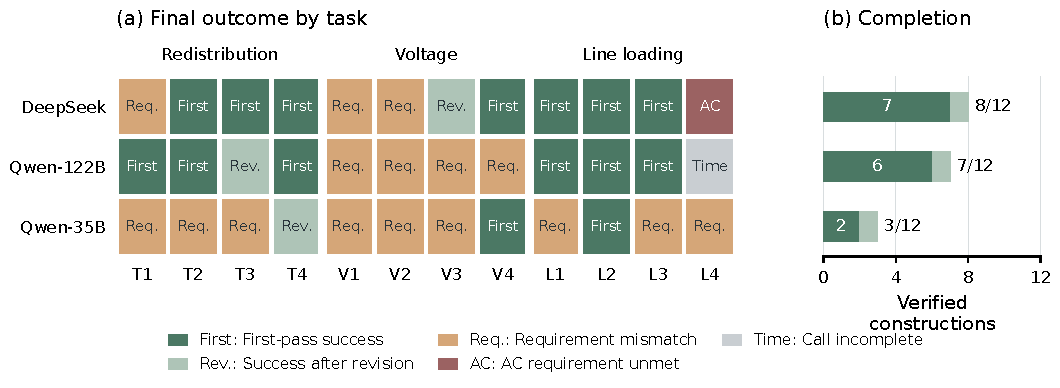
\includegraphics[width=\linewidth]{figures/fig5_backbone_applicability.pdf}
\caption{Per-task results and completion counts for the original three-API comparison. Requirement mismatches, incomplete calls, and AC rejections are reported separately. DeepSeek retains the original fixed-batch results; Qwen uses additional calls on the same requests. Shared AC observations are not counted as additional physical trials.}
\label{fig:backends}
\end{figure}

In the original three-API comparison, T2, V3, and L3 were evaluated three times per LLM, including their main runs. DeepSeek and Qwen-122B each completed T2 and L3 three times. DeepSeek completed V3 after format revision in all three runs, whereas neither Qwen model completed that request. Qwen-35B completed L3 in one of three runs after repair. Its three T2 outcomes were a requirement mismatch, a communication interruption, and an unresolved requirement check. These repetitions expose variation and recurring interpretation errors; they do not provide a statistical reliability estimate.

The historical Qwen main runs and three-model repetitions produce 21 candidates from accepted requirement specifications. Twenty exactly match archived physical observations; Qwen-122B T1 requires one new AC observation and passes the original requirements. Reuse is possible because parameter calculation is deterministic for the same expanded problem and complete matching conditions are checked before archived results are accepted.

For T2, V3, and L3, all three Codex runs completed on the first attempt. Each task produced the same checked constraints and complete load-factor vector across its three runs. Run~1 was already included in the main results, so these repetitions add six runs, giving eighteen formal runs in total. This is limited consistency evidence for three requests. It is not a general reliability estimate or a repeated independent power-flow experiment.

The eighteen generated requirement specifications each drove a new adjustment calculation. Sixteen resulting candidates matched archived physical observations under the full matching rules; V1 and V2 required two new independent observations, with six AC calculations including the baseline and restoration states. All applicable restoration checks passed. Thus all accepted tasks have physical support, while archived reuse is kept separate from new physical executions.


\section{Codex supplement protocol}
\label{app:codex-protocol}

The supplement used official Codex CLI~0.163.0 with ChatGPT authentication, requested model \texttt{gpt-6.1-sol}, and medium reasoning effort. Archived system and user message contents were preserved in order and marked by their original roles within one submitted input. This preserves the supplied text but not the original role hierarchy: the client adds its own instructions. No forced output format was used, and ordinary final answers were passed to the original parser. Each run began in a new empty working directory and a fresh temporary session. Tool features were disabled, and no tool-call events were observed in either the formal runs or the tool-challenge check. The records cannot establish every service-side instruction or the complete internal request sequence.

The external process deadline was 180~s. No equivalent was claimed for the historical 60~s network-idle limit, temperature~0, top-$p=1$, 4096-token output limit, or disabled reasoning. The returned events did not identify an exact model snapshot. No visible model substitution was observed, but the requested identifier should not be treated as confirmation of the returned model version. Forty-two frozen numerical and validation dependencies and one dynamically loaded historical helper matched their archived versions. No new equivalence rules, manual edits to generated specifications, or numerical feedback correction were introduced.

The twelve main runs were followed by two additional runs each for T2, V3, and L3. Compatibility probes remain outside all task denominators. Physical observations were reused only when the full candidate settings and relevant baseline, model, control, and power-flow context matched. Each new specification was checked against its own requirements and the original task. The two new physical observations were for V1 and V2; the other sixteen runs used archived observations. Counts of client starts, transport reconnections, numerical solves, AC calculations, and independent observations are therefore reported separately.

\FloatBarrier
\section{Incremental execution costs}
\label{app:costs}

Table~\ref{tab:costs} distinguishes new calls and AC calculations from reused observations. The allocation supplement includes two new LLM-driven constructions and two additional proportional-allocation observations; its first-level E/D observations are reused. The alternative-LLM study includes additional main runs and repeated runs but excludes the original DeepSeek main batch. Unknown token usage is left unknown rather than set to zero. Token totals from different LLMs are reported as service usage and are not treated as monetary costs.

\begin{table}[htbp]
\caption{Recorded incremental costs. PowerFactory session durations include connection, checks, extraction, and restoration. Local sensitivity acquisition is separate preparation work.}
\label{tab:costs}
\small
\begin{tabularx}{\linewidth}{@{}Xrrr@{}}
\toprule
Measure & Primary 12 tasks & Allocation supplement & \makecell{API model/repeat\\extension} \\
\midrule
New LLM requests & 13 & 2 & $51+2$ probes \\
Known total tokens & 95,206 & 18,538 & 395,864 \\
Requests with unknown usage & 0 & 0 & 2 \\
Adjustment calculations & 9 & 2 & 21 \\
New independent candidate observations & 9 & 4 & 1 \\
New AC calculations & 27 & 12 & 3 \\
Recorded API duration (s) & 305.5 & 46.8 & 2058.6$^{a}$ \\
Recorded PF-session duration (s) & 2650.6 & 1448.5 & 517.3 \\
\bottomrule
\end{tabularx}
\par\smallskip\footnotesize $^{a}$Formal calls only; compatibility-probe time is separate. The primary execution window was 2960.9~s, and the LLM extension window was 2607.3~s. These windows include overlapping API/PF duration measures and must not be summed with them.
\end{table}

\begin{table}[htbp]
\caption{Additional study blocks. Counts refer to the indicated batch, not total development cost. A client start is not a known number of underlying service requests.}
\label{tab:additional-costs}
\small
\begin{tabularx}{\linewidth}{@{}Xrrr@{}}
\toprule
Measure & Generation--load cases & Development pairs & Codex supplement \\
\midrule
Formal generation attempts & 4 API calls & 8 API calls & 18 client starts \\
Separate compatibility probes & 1 & 0 & 2 \\
Formal reported tokens & 30,520 & 58,534 & 284,355 \\
Probe tokens & 21 & 0 & 36,737 \\
Adjustment calculations & 3$^{a}$ & 8 & 18 \\
New independent candidate observations & 2 & 2 & 2 \\
New AC calculations & 6 & 6 & 6 \\
\bottomrule
\end{tabularx}
\par\smallskip\footnotesize $^{a}$S-T first and corrected candidates, plus S-L. One additional offline reference-correction solve is preparation. The representation study separately records four preparation solves.
\end{table}

The earlier generation--load batch contains three incomplete calls with unknown token usage and 21 AC calculations including preparation; these are retained separately. The closeout records 30,541 tokens including its 21-token probe. The Codex formal output total of 19,431 tokens includes 1,516 reasoning tokens, and its input total is 264,924. Its 72 visible transport reconnections are not specification revisions or independent case results. The underlying service-request count and monetary charges are unknown. The recorded 2033.015~s sum of client-process durations includes transport recovery and is nested within the 2848.292~s batch duration; it is not comparable to a pure model or power-flow execution time.


\FloatBarrier

\end{document}
